\documentclass[conference]{IEEEtran}
\usepackage{booktabs}
\usepackage{graphicx}
\usepackage{amsmath}
\usepackage{url}
\usepackage[hidelinks]{hyperref}
\graphicspath{{../results/figures/}}
\IfFileExists{generated/numbers.tex}{\newcommand{\SIIFinalQWK}{0.827}
\newcommand{\SIIFinalAcc}{0.771}
\newcommand{\SIIFinalMF}{0.473}
\newcommand{\SIIFinalMinRec}{0.148}
\newcommand{\SIIFinalSevRec}{0.00}
\newcommand{\SIIFinalPDRRec}{0.30}
\newcommand{\SIIFinalMildRec}{0.23}
\newcommand{\SIIBestQWK}{0.827}
\newcommand{\SIIBestAcc}{0.771}
\newcommand{\SIIBestMF}{0.473}
\newcommand{\SIIBestMinRec}{0.148}
\newcommand{\SIIBestSevRec}{0.00}
\newcommand{\SIIBestPDRRec}{0.30}
\newcommand{\SIIBestMildRec}{0.23}
\newcommand{\SIIVoteQWK}{0.788}
\newcommand{\SIIVoteAcc}{0.767}
\newcommand{\SIIVoteMF}{0.412}
\newcommand{\SIIVoteMinRec}{0.000}
\newcommand{\SIIVoteSevRec}{0.00}
\newcommand{\SIIVotePDRRec}{0.00}
\newcommand{\SIIVoteMildRec}{0.29}
\newcommand{\SIIMeanQWK}{0.791}
\newcommand{\SIIMeanAcc}{0.769}
\newcommand{\SIIMeanMF}{0.416}
\newcommand{\SIIMeanMinRec}{0.000}
\newcommand{\SIIMeanSevRec}{0.00}
\newcommand{\SIIMeanPDRRec}{0.00}
\newcommand{\SIIMeanMildRec}{0.30}
\newcommand{\SIIlowFinalQWK}{0.862}
\newcommand{\SIIlowFinalAcc}{0.798}
\newcommand{\SIIlowFinalMF}{0.603}
\newcommand{\SIIlowFinalMinRec}{0.370}
\newcommand{\SIIlowFinalSevRec}{0.17}
\newcommand{\SIIlowFinalPDRRec}{0.57}
\newcommand{\SIIlowFinalMildRec}{0.46}
\newcommand{\SIIlowBestQWK}{0.887}
\newcommand{\SIIlowBestAcc}{0.815}
\newcommand{\SIIlowBestMF}{0.630}
\newcommand{\SIIlowBestMinRec}{0.428}
\newcommand{\SIIlowBestSevRec}{0.31}
\newcommand{\SIIlowBestPDRRec}{0.55}
\newcommand{\SIIlowBestMildRec}{0.39}
\newcommand{\SIIlowVoteQWK}{0.887}
\newcommand{\SIIlowVoteAcc}{0.822}
\newcommand{\SIIlowVoteMF}{0.613}
\newcommand{\SIIlowVoteMinRec}{0.347}
\newcommand{\SIIlowVoteSevRec}{0.10}
\newcommand{\SIIlowVotePDRRec}{0.59}
\newcommand{\SIIlowVoteMildRec}{0.43}
\newcommand{\SIIlowMeanQWK}{0.887}
\newcommand{\SIIlowMeanAcc}{0.820}
\newcommand{\SIIlowMeanMF}{0.611}
\newcommand{\SIIlowMeanMinRec}{0.347}
\newcommand{\SIIlowMeanSevRec}{0.10}
\newcommand{\SIIlowMeanPDRRec}{0.59}
\newcommand{\SIIlowMeanMildRec}{0.43}
\newcommand{\FullFinalQWK}{0.808}
\newcommand{\FullFinalAcc}{0.785}
\newcommand{\FullFinalMF}{0.536}
\newcommand{\FullFinalMinRec}{0.159}
\newcommand{\FullFinalSevRec}{0.07}
\newcommand{\FullFinalPDRRec}{0.25}
\newcommand{\FullFinalMildRec}{0.55}
\newcommand{\FullBestQWK}{0.858}
\newcommand{\FullBestAcc}{0.780}
\newcommand{\FullBestMF}{0.512}
\newcommand{\FullBestMinRec}{0.211}
\newcommand{\FullBestSevRec}{0.10}
\newcommand{\FullBestPDRRec}{0.32}
\newcommand{\FullBestMildRec}{0.21}
\newcommand{\FullVoteQWK}{0.846}
\newcommand{\FullVoteAcc}{0.796}
\newcommand{\FullVoteMF}{0.527}
\newcommand{\FullVoteMinRec}{0.205}
\newcommand{\FullVoteSevRec}{0.00}
\newcommand{\FullVotePDRRec}{0.41}
\newcommand{\FullVoteMildRec}{0.38}
\newcommand{\FullMeanQWK}{0.839}
\newcommand{\FullMeanAcc}{0.796}
\newcommand{\FullMeanMF}{0.527}
\newcommand{\FullMeanMinRec}{0.193}
\newcommand{\FullMeanSevRec}{0.00}
\newcommand{\FullMeanPDRRec}{0.39}
\newcommand{\FullMeanMildRec}{0.39}
\newcommand{\FulllowFinalQWK}{0.858}
\newcommand{\FulllowFinalAcc}{0.809}
\newcommand{\FulllowFinalMF}{0.610}
\newcommand{\FulllowFinalMinRec}{0.388}
\newcommand{\FulllowFinalSevRec}{0.21}
\newcommand{\FulllowFinalPDRRec}{0.57}
\newcommand{\FulllowFinalMildRec}{0.34}
\newcommand{\FulllowBestQWK}{0.860}
\newcommand{\FulllowBestAcc}{0.813}
\newcommand{\FulllowBestMF}{0.599}
\newcommand{\FulllowBestMinRec}{0.342}
\newcommand{\FulllowBestSevRec}{0.28}
\newcommand{\FulllowBestPDRRec}{0.41}
\newcommand{\FulllowBestMildRec}{0.27}
\newcommand{\FulllowVoteQWK}{0.879}
\newcommand{\FulllowVoteAcc}{0.822}
\newcommand{\FulllowVoteMF}{0.623}
\newcommand{\FulllowVoteMinRec}{0.359}
\newcommand{\FulllowVoteSevRec}{0.17}
\newcommand{\FulllowVotePDRRec}{0.55}
\newcommand{\FulllowVoteMildRec}{0.39}
\newcommand{\FulllowMeanQWK}{0.882}
\newcommand{\FulllowMeanAcc}{0.825}
\newcommand{\FulllowMeanMF}{0.629}
\newcommand{\FulllowMeanMinRec}{0.370}
\newcommand{\FulllowMeanSevRec}{0.17}
\newcommand{\FulllowMeanPDRRec}{0.57}
\newcommand{\FulllowMeanMildRec}{0.39}
}{}

\begin{document}
\title{Reproducing Transfer-Learning and Snapshot-Ensemble Diabetic Retinopathy Grading on APTOS 2019:\\
Stage 2 (Base Paper \& Reproducibility Check) and Stage 3 (Baseline Reproduction)}
\author{\IEEEauthorblockN{Shivansh, Divyanshi, Vivek, Shubham}
\IEEEauthorblockA{CV Research-Reproduction Project --- Diabetic Retinopathy Grading}}
\maketitle

\begin{abstract}
We select Chilukoti \emph{et al.} (2024), which reports a quadratic weighted kappa (QWK) of 0.954 on APTOS~2019
with an ImageNet-initialised EfficientNet-B3 and 0.967 with EyePACS pre-training and snapshot ensembling, as
our base paper, document its reproducibility, and re-implement it from the text because no code is public.
We run the exact published protocol (300\,px, 60 epochs, batch 16) on a Colab T4 GPU, after compute-limited
pilot runs (224\,px, 30 epochs) on an Apple M2. With the paper's hyper-parameters the best-validation model
reaches test QWK \FullBestQWK{} and the 10-snapshot vote \FullVoteQWK{}, about 0.10 below the reported 0.954.
Training at lr $10^{-3}$ is unstable at both resolutions, and Severe NPDR is almost never recognised (recall
$\leq$\FullBestSevRec{}). Changing only the learning rate to $10^{-4}$ makes training stable and gives QWK
\FulllowMeanQWK{} for the snapshot ensemble, with PDR recall rising to \FulllowMeanPDRRec{}. The full resolution
and schedule add about 0.03 QWK at the paper's learning rate but nothing at $10^{-4}$, so a gap of about 0.07
remains that none of the stated settings explain. We also find 123 groups of byte-identical images in APTOS
(30 with conflicting grades), whose leakage into the test set has no measurable effect. No clinical claims are made.
\end{abstract}

\section{Stage 2: Base Paper and Reproducibility Check}

\subsection{Selected base paper}
We reproduce Chilukoti \emph{et al.}, ``A reliable diabetic retinopathy grading via transfer learning and
ensemble learning with quadratic weighted kappa metric,'' \emph{BMC Medical Informatics and Decision
Making}, 24:37, 2024~\cite{chilukoti2024}. The paper fine-tunes an ImageNet-pretrained EfficientNet-B3 with a
three-layer classifier head, pre-processes fundus images with CLAHE followed by Gaussian blur, and ensembles
predictions from weights saved at several epochs of a single training run (``snapshot'' ensembling). It reports
QWK as the primary metric: 0.954 on APTOS~2019 for a single model trained from ImageNet weights, and 0.967
when the model is first trained on EyePACS and the snapshot ensemble is used.

\subsection{Why this paper}
It matches the direction set by our literature review: it treats QWK (an ordinal, imbalance-aware agreement
metric) as primary, uses a transfer-learning CNN that fits free-tier hardware, evaluates on the public
five-class APTOS~2019 dataset, and leaves the two gaps we identified untouched: no imbalance-aware loss and
no ordinal-aware training objective. That makes it a clean base for a single-variable Stage~4 hypothesis.

\subsection{Reproducibility checklist}
\begin{table}[h]
\centering
\caption{Reproducibility checklist for the base paper.}
\label{tab:checklist}
\footnotesize
\begin{tabular}{p{0.30\columnwidth}p{0.62\columnwidth}}
\toprule
Item & Our answer \\
\midrule
Public code? & No. No repository is linked and none was found on GitHub; we re-implemented the method from the
paper text (Sec.~\ref{sec:protocol}). \\
Dataset public \& size? & Yes. APTOS 2019 Blindness Detection (Kaggle), 3{,}662 labelled fundus images,
$\approx$8.9\,GB at full resolution; obtained from a full-resolution Hugging Face mirror
(\texttt{sngsfydy/aptos}). Class counts 1805/370/999/193/295. \\
Fits free GPU? & Yes. The exact protocol (300$\times$300, batch 16, 60 epochs) takes $\approx$1.3\,h on a
free Colab T4. Locally (Apple M2, 8\,GB unified memory) B3 at 300\,px swaps heavily even at batch 8, so the
local pilot uses 224\,px. \\
Last commit / usable? & Not applicable (no code). Our implementation: PyTorch 2.14, \texttt{timm} 1.0.30. \\
Metric defined? & Yes. QWK (primary), plus accuracy, precision, recall, F1, AUC-ROC. We additionally report
macro-F1, per-class precision/recall/F1, macro one-vs-rest AUC and the confusion matrix. \\
Split defined? & Partially. A 70/15/15 train/val/test split is stated for EyePACS only; not stated for APTOS.
We use a stratified 70/15/15 split with a fixed seed. \\
Hyper-parameters? & Partially. Adam, lr $10^{-3}$, weight decay $10^{-4}$, gradient clipping 0.1, 60 epochs
(strategy~1). Batch size, APTOS epoch count, loss function, CLAHE parameters and blur kernel are not stated. \\
\bottomrule
\end{tabular}
\end{table}

\subsection{Under-specified details and our choices}
\begin{itemize}
\item \textbf{Loss:} not stated; softmax output implies cross-entropy, which we use.
\item \textbf{Gradient clipping ``0.1'':} interpreted as global L2-norm clipping at 0.1.
\item \textbf{CLAHE / blur:} clip limit 2.0, 8$\times$8 tiles on the LAB luminance channel, then a
5$\times$5 Gaussian blur, applied identically to train, validation and test images.
\item \textbf{Resize:} plain square resize (no border cropping), as the paper mentions only resizing.
\item \textbf{Augmentation:} none beyond CLAHE and blur, which the paper calls ``augmentation'' but which act as
deterministic pre-processing.
\item \textbf{Ensemble:} strategy~2 takes the majority vote over predictions from 10 evenly spaced
snapshots; strategy~1 averages the 30- and 60-epoch (here: mid- and final-epoch) snapshots.
\item \textbf{Reported model:} the paper does not say whether the final-epoch or best-validation model is
evaluated; we report both.
\end{itemize}

\subsection{Red flags noted before reproduction}
Several reported numbers are internally inconsistent, which we flag as context for the reproduction gap:
(i) in Table~3 of~\cite{chilukoti2024}, precision, recall and QWK of the B3 ensemble are all exactly 0.867,
and models predicting only class~0 report a macro AUC of 0.196, below the 0.5 that a constant predictor
yields; (ii) in Table~6, accuracy, precision, recall and F1 agree to within 0.01 on an imbalanced dataset;
(iii) the APTOS split is not described, so overlap between near-duplicate images in train and test (a
known APTOS issue) cannot be ruled out. We audit duplicates ourselves in Sec.~\ref{sec:dups}.

\section{Stage 3: Reproduction Protocol}
\label{sec:protocol}

\subsection{Data}
APTOS~2019~\cite{aptos2019} contains 3{,}662 labelled colour fundus photographs from Aravind Eye Hospital
graded 0--4 (No DR 1805, Mild 370, Moderate 999, Severe 193, PDR 295). Images were stored at a 512\,px longest
side (aspect ratio preserved) and resized at load time. We use a stratified 70/15/15 split with seed 42
(2{,}562/550/550 images).

\subsection{Duplicate audit}
\label{sec:dups}
Hashing the raw bytes revealed 123 groups of byte-identical images (128 redundant rows); in 30 of these groups
the copies carry \emph{different} grades (e.g.\ the same photograph labelled Moderate and PDR). Under a naive
random split, 29 of the 550 test images (5.3\%) have an identical copy in the training set, and 5 of them with
a conflicting grade. We train on the \textbf{faithful} split (all 3{,}662 rows, as the paper presumably did)
and quantify the effect of this leakage by re-scoring each model on the 521 test images that have no copy in
the training set (Sec.~\ref{sec:gap}). A de-duplicated protocol (conflicting groups removed, one copy per
group: 3{,}504 images) is implemented for Stage~5.

\subsection{Model and training}
Following~\cite{chilukoti2024}: an ImageNet-pretrained EfficientNet-B3~\cite{tan2019efficientnet}
(\texttt{timm}) with global average pooling (1{,}536-d) feeds a head of FC(512), Dropout(0.5), ReLU,
FC(512), Dropout(0.25), ReLU and FC(5). The whole network is
fine-tuned with Adam (lr $10^{-3}$, weight decay $10^{-4}$), global gradient-norm clipping at 0.1 and
cross-entropy loss. Inputs are normalised with ImageNet statistics.

\textbf{Strategy 2 (headline):} CLAHE~\cite{zuiderveld1994clahe} on the LAB luminance channel (clip 2.0,
8$\times$8 tiles), 5$\times$5 Gaussian blur, square resize. Predictions are taken from 10 evenly spaced epochs
and combined by majority vote. \textbf{Strategy 1:} plain resize to 150\,px; predictions from the mid-point
and final epochs are averaged.

\subsection{Compute and run configurations}
\textbf{Exact protocol (headline).} Strategy~2 exactly as published: 300$\times$300 inputs, batch size 16,
60 epochs, snapshots every 6 epochs. These runs used a free Google Colab NVIDIA T4 GPU (CUDA, full fp32
precision, no mixed precision), took 78\,s per epoch ($\approx$1.3\,h per run) and finished without interruption.
Checkpoints were written to Google Drive after every epoch so that a disconnected session could resume.

\textbf{Compute-limited pilot.} Before GPU access, we trained on an Apple M2 with 8\,GB unified memory (PyTorch
MPS backend). EfficientNet-B3 at 300\,px exceeded the memory budget even at batch size 8 (steps took 25--45\,s
because of swapping), so the pilot used \textbf{224\,px, batch size 8 and 30 epochs} (snapshots every 3 epochs),
$\approx$2\,h per run. The paper-setting pilot was interrupted once (disk full while writing a checkpoint) and
resumed from its epoch-13 checkpoint. We keep the pilot runs because comparing them with the exact protocol
isolates the effect of resolution and schedule (Sec.~\ref{sec:res}).

All four runs share the same split (seed 42), model seed and code. Each configuration is trained once with the
paper's learning rate ($10^{-3}$) and once with $10^{-4}$ (diagnostic, Sec.~\ref{sec:diag}).
The EyePACS-pretraining variant behind the paper's 0.967 was not attempted: EyePACS is
35{,}126 images ($\approx$10$\times$ APTOS), which is beyond our compute budget, so our target is the
paper's ImageNet-initialised result (QWK 0.954).

\subsection{Metrics}
Following the course rules and our literature review, we report QWK~\cite{cohen1968kappa} (primary), accuracy,
macro-F1, macro one-vs-rest AUC, per-class precision/recall/F1, ``minority recall'' (mean recall of Severe
and PDR), the number of test predictions off by two or more grades, and confusion matrices. We report the
final-epoch model, the best-validation-QWK model, and both snapshot-ensemble variants.

\IfFileExists{sections/results.tex}{\section{Stage 3: Results}
\label{sec:results}

\IfFileExists{generated/main_table.tex}{\begin{table*}[t]
\centering
\caption{Reproduced test-set results on APTOS 2019 (550 test images, faithful split). Paper: QWK 0.954 (single model, ImageNet init) and 0.967 (EyePACS init + snapshot ensemble).}
\label{tab:main}
\footnotesize
\begin{tabular}{llcccccc}
\toprule
Configuration & Prediction & QWK & Acc. & Macro-F1 & Macro AUC & Minority recall & $|\Delta|\geq2$ errors \\
\midrule
300\,px/60 ep, lr $10^{-3}$ (paper) & final epoch & 0.808 & 0.785 & 0.536 & 0.887 & 0.159 & 37 \\
 & best val QWK & 0.858 & 0.780 & 0.512 & 0.914 & 0.211 & 31 \\
 & snapshot vote & 0.846 & 0.796 & 0.527 & 0.923 & 0.205 & 37 \\
 & snapshot mean & 0.839 & 0.796 & 0.527 & 0.923 & 0.193 & 38 \\
\midrule
300\,px/60 ep, lr $10^{-4}$ & final epoch & 0.858 & 0.809 & 0.610 & 0.899 & 0.388 & 40 \\
 & best val QWK & 0.860 & 0.813 & 0.599 & 0.908 & 0.342 & 27 \\
 & snapshot vote & 0.879 & 0.822 & 0.623 & 0.934 & 0.359 & 29 \\
 & snapshot mean & 0.882 & 0.825 & 0.629 & 0.934 & 0.370 & 28 \\
\midrule
224\,px/30 ep, lr $10^{-3}$ (M2) & final epoch & 0.827 & 0.771 & 0.473 & 0.897 & 0.148 & 48 \\
 & best val QWK & 0.827 & 0.771 & 0.473 & 0.897 & 0.148 & 48 \\
 & snapshot vote & 0.788 & 0.767 & 0.412 & 0.913 & 0.000 & 50 \\
 & snapshot mean & 0.791 & 0.769 & 0.416 & 0.913 & 0.000 & 49 \\
\midrule
224\,px/30 ep, lr $10^{-4}$ (M2) & final epoch & 0.862 & 0.798 & 0.603 & 0.897 & 0.370 & 30 \\
 & best val QWK & 0.887 & 0.815 & 0.630 & 0.894 & 0.428 & 24 \\
 & snapshot vote & 0.887 & 0.822 & 0.613 & 0.930 & 0.347 & 27 \\
 & snapshot mean & 0.887 & 0.820 & 0.611 & 0.930 & 0.347 & 27 \\
\bottomrule
\end{tabular}
\end{table*}
}{}
\IfFileExists{generated/per_class_table.tex}{\begin{table}[t]
\centering
\caption{Per-class test metrics, exact paper protocol (300\,px, 60 epochs, lr $10^{-3}$).}
\label{tab:perclass}
\footnotesize
\begin{tabular}{llcccc}
\toprule
Grade & Model & Prec. & Recall & F1 & $n$ \\
\midrule
No DR & best val & 0.97 & 0.96 & 0.96 & 271 \\
Mild & best val & 0.44 & 0.21 & 0.29 & 56 \\
Moderate & best val & 0.65 & 0.93 & 0.76 & 150 \\
Severe & best val & 0.27 & 0.10 & 0.15 & 29 \\
PDR & best val & 0.52 & 0.32 & 0.39 & 44 \\
\midrule
No DR & snapshot vote & 0.94 & 0.97 & 0.96 & 271 \\
Mild & snapshot vote & 0.50 & 0.38 & 0.43 & 56 \\
Moderate & snapshot vote & 0.70 & 0.91 & 0.79 & 150 \\
Severe & snapshot vote & 0.00 & 0.00 & 0.00 & 29 \\
PDR & snapshot vote & 0.53 & 0.41 & 0.46 & 44 \\
\bottomrule
\end{tabular}
\end{table}
}{}

\subsection{Faithful reproduction (exact protocol)}
Table~\ref{tab:main} summarises the test results. With the paper's protocol and hyper-parameters, the
best-validation model (epoch 15) reaches QWK~\FullBestQWK{} (accuracy \FullBestAcc{}, macro-F1 \FullBestMF{}),
against 0.954 reported in~\cite{chilukoti2024}: a gap of about 0.10 QWK. The final-epoch model is weaker
(QWK \FullFinalQWK{}). The 10-snapshot majority vote, the paper's central contribution, gives \FullVoteQWK{}:
better than the final epoch but below the best single checkpoint.

Training was unstable (Fig.~\ref{fig:curves}, Fig.~\ref{fig:compare}): validation QWK fell below 0.75 at
epochs 3, 5, 8, 10, 17, 22, 23 and 36 (to 0.556 at epoch 36) and recovered within one or two epochs, and the
best validation score (0.895 at epoch 15) was never reached again. Test QWK of the individual snapshots
(epochs 6, 12, \dots, 60) was 0.830, 0.770, 0.828, 0.834, 0.803, 0.522, 0.808, 0.773, 0.781 and 0.808. The
members are of uneven quality and one is very poor, so the vote cannot exceed the best member. Snapshot
ensembling assumes comparably good, diverse members~\cite{huang2017snapshot}, which an unstable trajectory
without a cyclic learning-rate schedule does not provide.

\begin{figure}[t]
\centering
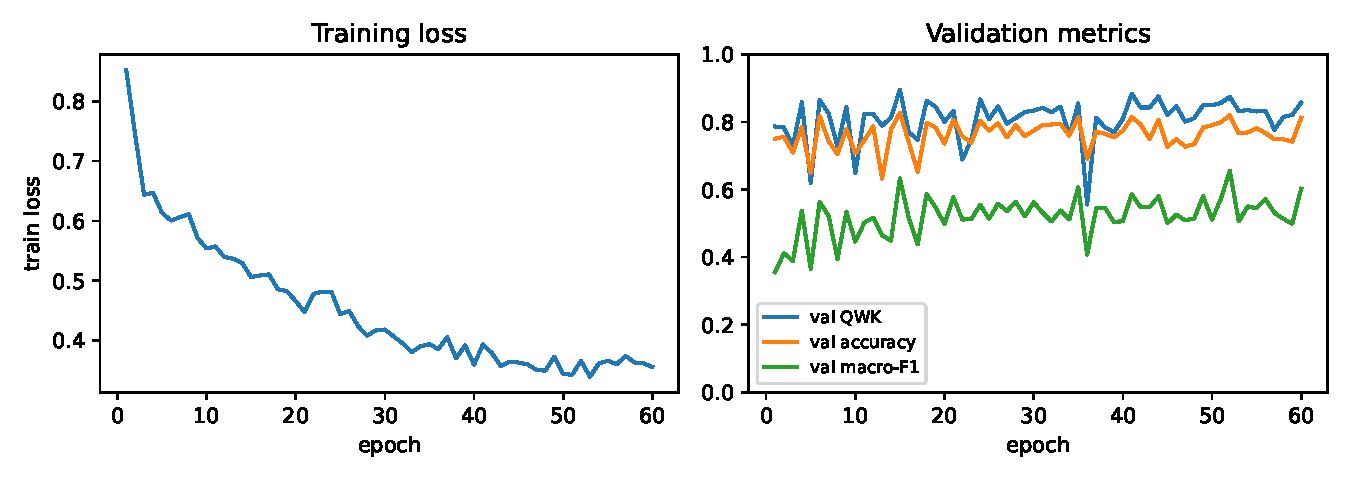
\includegraphics[width=\columnwidth]{s2_paper300_curves.pdf}
\caption{Training loss and validation metrics, exact protocol with the paper's lr $10^{-3}$.}
\label{fig:curves}
\end{figure}

\subsection{Per-grade behaviour}
QWK and accuracy hide a severe minority-grade failure (Table~\ref{tab:perclass}, Fig.~\ref{fig:cm}).
No DR (recall 0.96) and Moderate (0.93) are learned well, but \textbf{Severe NPDR is almost never recognised}:
3 of 29 Severe eyes for the single model, 0 for the vote, and at most 5 in any snapshot. PDR recall is
\FullBestPDRRec{} (single model) and \FullVotePDRRec{} (vote), and Mild recall only \FullBestMildRec{}.
Severe cases are mostly called Moderate (17/29) or PDR (9/29), 24 of 44 PDR eyes are called Moderate, and
34 of 56 Mild eyes are called Moderate. The errors are mostly adjacent-grade, which is why QWK stays near
0.86 even though two of five grades are essentially unrecognised; this is exactly the ``accuracy (and even QWK)
can be misleading'' gap identified in our literature review.

\begin{figure}[t]
\centering
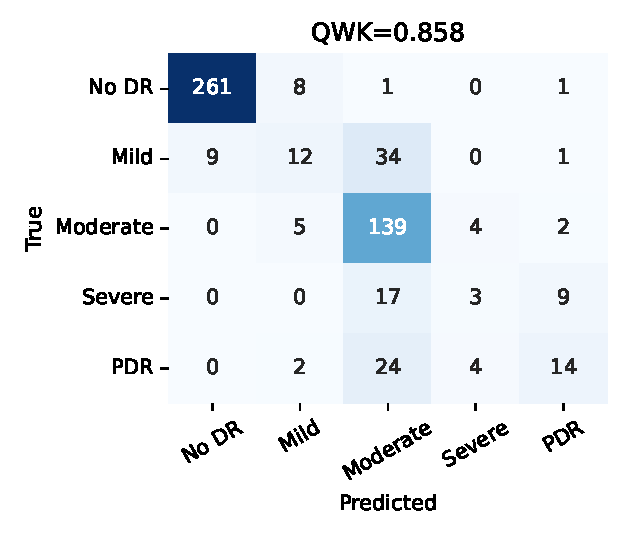
\includegraphics[width=0.78\columnwidth]{s2_paper300_best_val_cm.pdf}
\caption{Test confusion matrix of the reproduced single model (exact protocol, paper hyper-parameters).}
\label{fig:cm}
\end{figure}

\IfFileExists{sections/diagnostic.tex}{\subsection{Diagnostic: learning rate $10^{-4}$}
\label{sec:diag}
To test whether optimisation explains the gap, we repeated the exact protocol with a single change, lr
$10^{-3}\to10^{-4}$ (same split, seed, resolution, epochs and snapshots). Training became stable: validation QWK
stayed between 0.81 and 0.89 for all 60 epochs with no collapses (Fig.~\ref{fig:compare}), and training loss
fell to 0.12 by epoch 10 (0.55 at lr $10^{-3}$). The best-validation checkpoints are similar (QWK
\FulllowBestQWK{} vs.\ \FullBestQWK{}), but every other prediction improves: final epoch \FullFinalQWK{}$\to$\FulllowFinalQWK{},
snapshot vote \FullVoteQWK{}$\to$\FulllowVoteQWK{} and snapshot mean \FullMeanQWK{}$\to$\FulllowMeanQWK{}
(macro-F1 \FulllowMeanMF{}). Minority recall rises from \FullBestMinRec{} to \FulllowMeanMinRec{} (ensemble mean;
Severe \FulllowMeanSevRec{}, PDR \FulllowMeanPDRRec{}).

With stable training the snapshots are uniformly good (test QWK 0.823--0.885) and the ensemble now beats the
best single model, consistent with the snapshot-ensemble assumption that members are of comparable quality.
Severe NPDR remains the weakest grade (5 of 29 recognised by the ensemble; 16 called Moderate) and Mild is still
mostly confused with Moderate (26/56). The low training loss with a flat validation curve suggests the model
overfits after about 10 epochs, which a learning-rate schedule or stronger augmentation could address.
This run is the baseline we carry into Stage~4.

\subsection{Effect of resolution and schedule}
\label{sec:res}
Comparing the exact protocol with our compute-limited pilot isolates the effect of using 224\,px for 30 epochs
(Table~\ref{tab:main}, Fig.~\ref{fig:compare}). At lr $10^{-3}$ the full protocol helps: best single model
\SIIBestQWK{}$\to$\FullBestQWK{} and vote \SIIVoteQWK{}$\to$\FullVoteQWK{}, mostly because the vote is no longer
dragged down as far by collapsed snapshots. At lr $10^{-4}$ it does not: the pilot's best model and vote
(\SIIlowBestQWK{}, \SIIlowVoteQWK{}) are at least as good as the exact protocol's (\FulllowBestQWK{},
\FulllowVoteQWK{}). Resolution and schedule therefore account for at most $\approx$0.03 QWK, and the learning
rate matters more than either.

\begin{figure}[t]
\centering
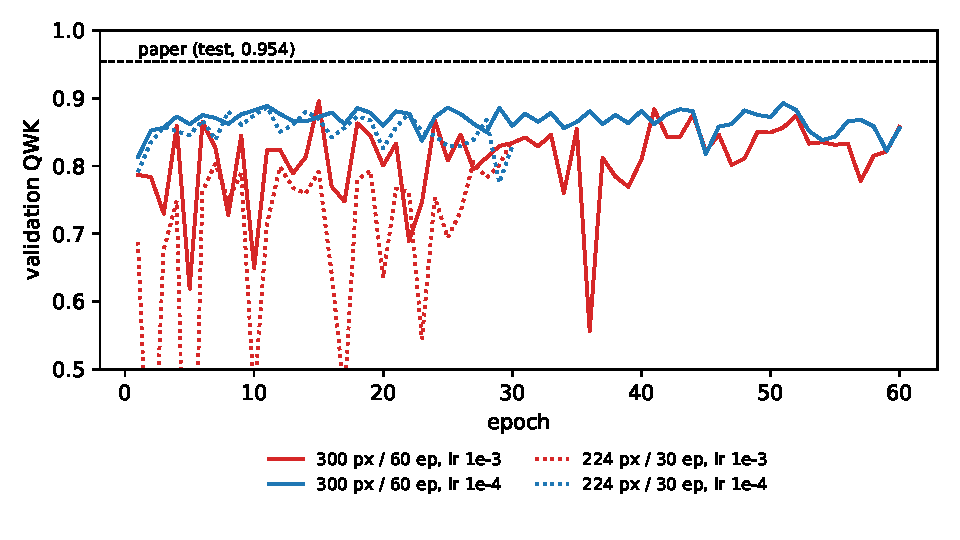
\includegraphics[width=\columnwidth]{val_qwk_compare.pdf}
\caption{Validation QWK per epoch for all four runs. lr $10^{-3}$ (red) is unstable at both resolutions;
lr $10^{-4}$ (blue) is stable. The dashed line is the paper's reported test QWK.}
\label{fig:compare}
\end{figure}
}{}

\subsection{Reproduction-gap analysis}
\label{sec:gap}
\begin{itemize}
\item \textbf{Duplicate leakage does not explain it.} Excluding the 29 test images with an identical copy in
training changes the single model's QWK from 0.858 to 0.862 (0.879 to 0.879 for the lr-$10^{-4}$ vote). The
leaked images are actually predicted \emph{worse} (58.6\% accuracy), because several copies carry conflicting grades.
\item \textbf{Optimisation (learning rate) explains part of it.} Full fine-tuning with Adam at $10^{-3}$ and
gradient clipping at 0.1 is unstable at both resolutions and batch sizes; lowering it to $10^{-4}$ removes the
collapses and improves the final-epoch and ensemble predictions by 0.03--0.05 QWK (Sec.~\ref{sec:diag}). The paper's own Table~3, where VGG and ResNet models
predict only class~0 under the same settings, is consistent with this.
\item \textbf{Resolution and schedule explain little.} Moving from our 224\,px / 30-epoch pilot to the exact
300\,px / 60-epoch protocol adds 0.03 QWK at lr $10^{-3}$ and nothing at $10^{-4}$ (Sec.~\ref{sec:res}).
\item \textbf{Unreported details.} The split, loss, CLAHE parameters, and whether the reported model is the
final or the best-validation one are not stated; each can move QWK by a few points on a 550-image test set.
\item \textbf{Reported numbers.} The internal inconsistencies noted in Sec.~2 (e.g.\ identical precision, recall
and QWK; macro AUC below 0.5) mean the reported 0.954 may itself not be reliable. With the stated protocol run
exactly, a gap of $\approx$0.07 QWK remains that none of the stated settings account for.
\end{itemize}

\subsection{Failure cases}
Fig.~\ref{fig:fail} shows the most confidently wrong test predictions of the exact-protocol model. Eight of the
ten are PDR eyes predicted as Mild or Moderate with high confidence, including one with a large pre-retinal
haemorrhage; the other two are a dim, low-contrast No DR image and a Mild image both predicted as PDR.
Neovascularisation is small and easy to miss, and the model appears to rely on exudates and overall image
appearance instead.

\begin{figure*}[t]
\centering
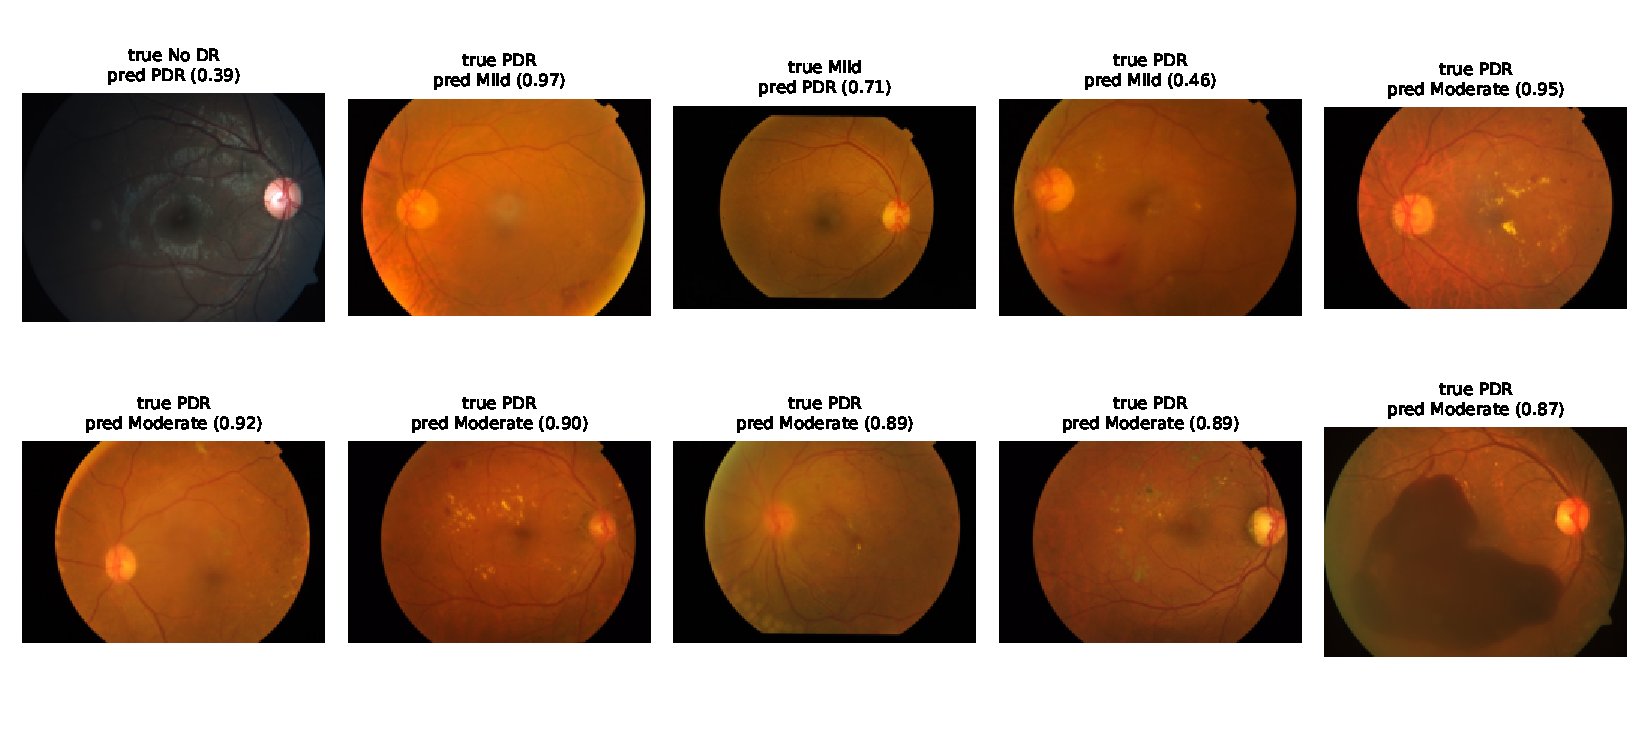
\includegraphics[width=0.9\textwidth]{s2_paper300_failures.pdf}
\caption{Ten largest-error test predictions of the reproduced single model, exact protocol (true grade,
predicted grade, confidence).}
\label{fig:fail}
\end{figure*}

\section{Limitations}
Single dataset (APTOS~2019) and a single seed per configuration; no external validation; the EyePACS-pretrained
configuration (0.967) was not reproduced. The 550-image test set contains only 29 Severe and 44 PDR images, so
per-grade recall estimates are noisy, and QWK differences of 0.01--0.02 between configurations are within
run-to-run variation. This is a reproduction study; no clinical claims are made.

\section{Next Step (Stage 4 preview)}
The reproduction shows that the paper's pipeline fails on exactly the grades that matter most clinically. Our
Stage~4 hypothesis will therefore change one variable, the training loss, from cross-entropy to a
class-balanced, ordinal-aware objective, on top of the stable lr-$10^{-4}$ exact-protocol baseline (snapshot
ensemble QWK \FulllowMeanQWK{}, Severe recall \FulllowMeanSevRec{}), and will be stated with a predicted
direction and magnitude before any code is run.
}{}

\bibliographystyle{IEEEtran}
\bibliography{refs}
\end{document}
